\section{Exercício 1}

O exercício um é o seguinte: Descobrir se um número \emph{n} positivo é múltiplo
de número do grupo +5(se por acaso, o valor de grupo + 5 ultrapassar o número do
maior grupo, deve ser subtraído o número do maior grupo.

O o grupo deste trabalho é o grupo 1, logo o exercicío será ver se um número é
divisível por 6.

\subsection{Descrição Alto Nível}

A desrição em alto nível foi utilizando a linguagem python é desta forma:

\begin{lstlisting}

def div(n, grupo):
    divisor = grupo + 5
    res = n
    while res >= grupo:
        res -= divisor
    
    return res

\end{lstlisting}

\subsection{Descrição Baixo nível}
\begin{verbatim}
    
.CODE
    lda grupo
    add #5
    not
    add #1
    sta divisor
    lda num
    sta resto
    ENQUANTO:
        lda resto
        add divisor
        jz  DIVIDE 
        jn  SOBRA
        sta resto
        jmp ENQUANTO
    SOBRA:
        lda #0
        sta resp
        jmp FIM
    DIVIDE:
        lda #1
        sta resp        
    FIM:
        hlt
.ENDCODE

.DATA
   num:     db  #12 ;Num a ser testado 
   resp:    db  #01
   grupo:   db  #1
   divisor: db  #0
   resto:   db  #0
.ENDDATA
\end{verbatim}

\subsection{Tela Montador}

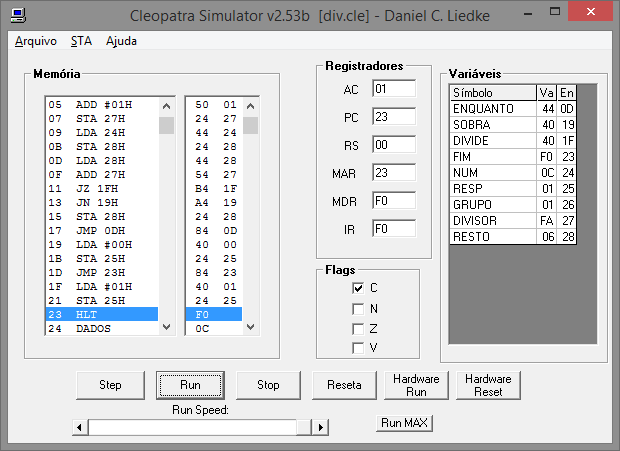
\includegraphics{images/div.png}

\subsection{Contagem Operações e estimativa de de tempo de execução}

Considerando \emph{num} como \emph{x} temos a seguinte função:
$$f(x) = 40x + 88$$

O Tempo de excução seria 0.000568ms para x=12 ao considerarmos que o Cleópatra
opera a 1GHz.
